\chapter{The ATLAS Experiment at the LHC}

	ATLAS (A Toroidal LHC ApparatuS) is one of the four main experiments (ATLAS, CMS, ALICE, LHCb) taking data at a center-of-mass energy of $13$ TeV using beams delivered by the Large Hadron Collider (LHC). In this chapter an overview of the LHC will be given in Section \ref{sec:lhc}, then the ATLAS detector will be described in Section \ref{sec:det}, and finally the Trigger system, used to cleverly store the data, will be described in Section \ref{sec:trigSyst}. A more in-depth description of the Trigger algorithms I have been involved in will be given in Chapter \ref{ch:trigger}.



	% --------------------------------
	% -------  THE LHC
	% --------------------------------
	\section{The LHC}
	\label{sec:lhc}
	
		As of today, the LHC is the world’s largest and most powerful particle accelerator. It was designed to help answer some of the fundamental open questions in particle physics by colliding protons at an unprecedented energy and luminosity. It is located at the European Organisation for Nuclear Research (CERN), in the Geneva area, at a depth ranging from 50 to 175 metres underground. It consists of a 27-kilometre ring made of superconducting magnets, and inside it two high-energy particle beams travel in opposite directions and in separate beam pipes. 

		The beams are guided around the ring by a strong magnetic field generated by coils - made of special electric cables - that can operate in a superconducting regime.%, being capable of conducting electricity almost without resistance or loss of energy. 
		1232 superconducting dipole and 392 quadrupole magnets, with an average magnetic field of 8.3 T, are employed and kept at a temperature below 1.7 K, in order to preserve their superconducting properties. The formers are used to bend the beams and the latters to keep them focused while they get accelerated. 
		%In order for this to be possible though, the magnets have to remain at a temperature of -271.3$^\circ$C for which a distribution system of liquid helium is employed.
		
		The collider first went live on September 2008 even though, due to a magnet quench incident that damaged over 50 superconducting magnets, it has been operational since November 2009 when low-energy beams circulated in the tunnel for the first time since the incident. This also marked the start of the main research programme and the beginning of the so-called Run 1: first operational run (2009 - 2013).


		%\subsection*{Performance of the LHC}
		\subsection*{Performance of the LHC}

			In June 2015 the LHC restarted delivering physics data, after a two-year break, the so-called Long Shutdown 1 (LS1), during which the magnets were upgraded to handle the current required to circulate 7-TeV beams. It was the beginning of the so-called Run 2 - second operational run (2015-2018) - during which LHC has collided up to $10^{11}$ bunches of protons every 25 ns at the design luminosity - the highest luminosiy the detector was designed to cope with - of $2 \cdot 10^{34} \mathrm{cm}^{-2}\mathrm{s}^{-1}$. The definiton of the luminosity is:

			\begin{equation}
				{\mathcal L} = f \frac{n_b N_1 N_2}{4 \pi \sigma_x \sigma_y}
			\label{eq:lumi}
			\end{equation}

			\noindent where $N_1$ and $N_2$ are the number of protons per bunch in each of the colliding beams, $f$ is the revolution frequency of the bunch collisions, $n_b$ the number of proton per bunch, and $\sigma_x$ and $\sigma_y$ are the horizontal and vertical dimensions of the beam. The luminosity is strictly related to the number of collisions occurring during a certain experiment via the following: 

			\begin{equation}
					{\mathcal N}_{\mathrm{event}} = {\mathcal L} \sigma_{\mathrm{event}}
			\label{eq:lumiEvt}
			\end{equation}

			\noindent where $\sigma_{\mathrm{event}}$ is the cross section of the process under investigation.  It has not only collided protons but also heavy ions, in particular lead nuclei at $\sqrt{s_{NN}} = 5.02$ TeV, at a luminosity of $10^{27} \mathrm{cm}^{-2} \mathrm{s}^{-1}$\cite{HI2015}.



		\subsection*{Acceleration stages}

			\begin{figure}[!htb]
				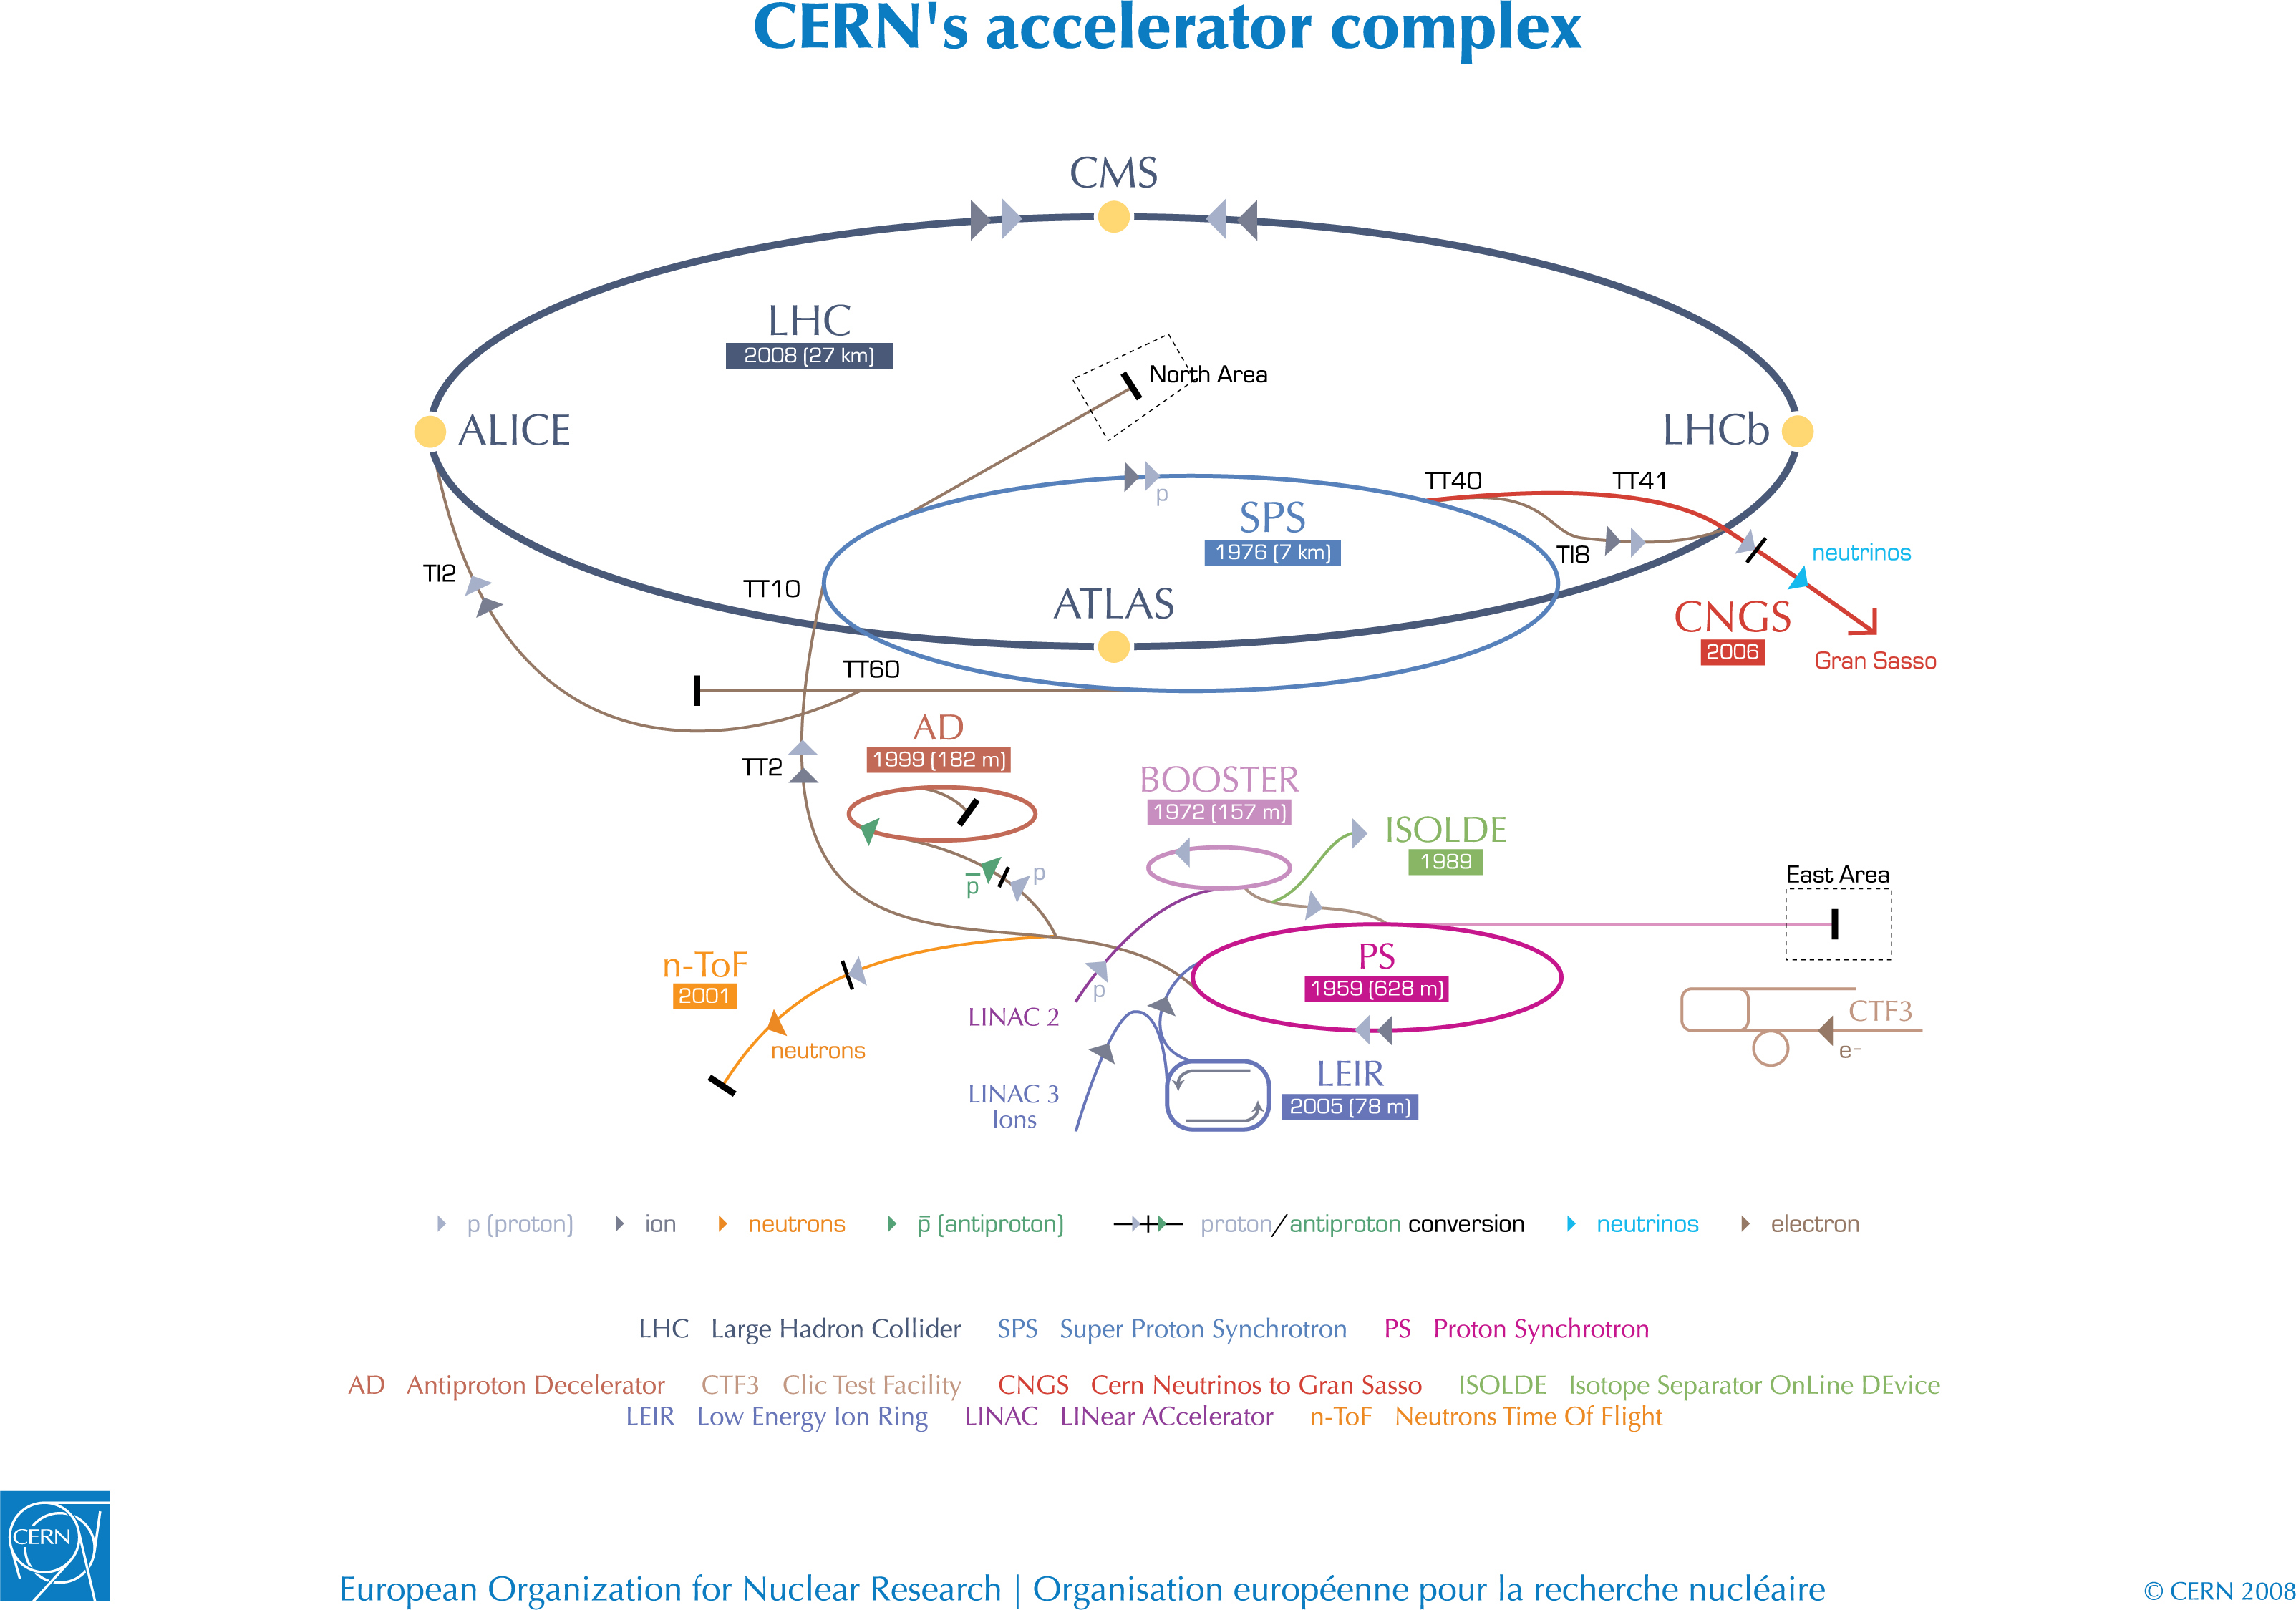
\includegraphics[width=\textwidth]{Detector/cern-acc-complex.jpg}
				\caption{CERN Accelerator complex. The LHC is the last ring (dark grey line). Smaller machines are used for early-stage acceleration and also to provide beams for other experiments \cite{Lefevre2008}.}
				\label{fig:cern-acc-complex}
			\end{figure}

			Before reaching the maximum energy, the proton beams are accelerated by smaller accelerators through various stages. Figure \ref{fig:cern-acc-complex} shows a sketch of the CERN's accelerator complex. It all begins at the linear accelerator LINAC 2. Here protons are accelerated up to 50 MeV, and then injected in the Proton Synchrotron Booster (PSB) where they reach 1.4 \GeV. The next stage is the Proton Synchrotron (PS), which boosts the beams up to 25 \GeV\, and then the Super Proton Synchrotron (SPS) makes them reach energies up to 450 \GeV. Eventually, the beams are injected in bunches with a 25 ns spacing into the LHC, where they travel in opposite directions, while they are accelerated to up to 13 TeV. Once the bunches reach the maximum energy, they are made collide at four different points, inside four experiments around the ring \cite{LHCDesignReport}. 

			The heavy ion beams acceleration procedure is slightly different. Their journey starts at LINAC 3 first, and the Low Energy Ion Ring (LEIR) then, before they make their way into the PS where they follow the same path as the protons \cite{LHCDesignReport}. 

			The four large detectors on the collision points are; the multi-purpose detectors A Toroidal LHC ApparatuS (ATLAS), and Compact Muon Solenoid (CMS) \cite{CMSJINST}, Large Hadron Collider beauty (LHCb) \cite{LHCb2008}, which focuses on flavour physics, and A Large Ion Collider Experiment (ALICE) \cite{ALICEJINST} which specialises in heavy ion physics. The \emph{big four} are not the only experiments at the CERN's accelerator complex. There also are smaller experiments based at the the four caverns about the collision points e.g. TOTEM, LHCf and MoEDAL, but this will not be discussed any further in this thesis.
		


	% --------------------------------
	% -------  THE DETECTOR
	% --------------------------------
	\section{The ATLAS Detector}
	\label{sec:det}

		\begin{figure}[!htb]
			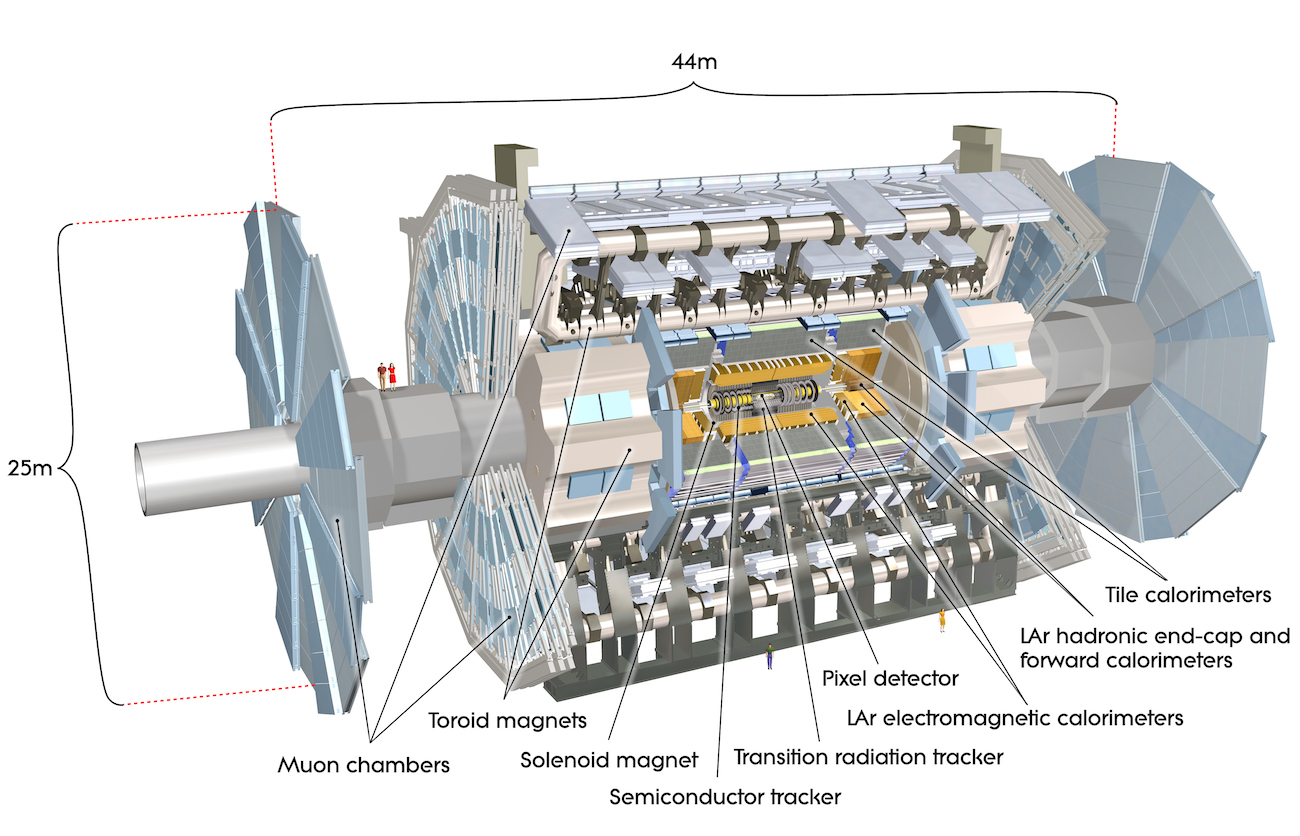
\includegraphics[width=\textwidth]{Detector/cut-away-det.jpg}
			\caption{Cut-away view of the ATLAS detector. The dimensions of the detector are 25 m in height and 44 m in length. The overall weight of the detector is approximately 7000 tonnes \cite{Lefevre2008}.}
			\label{fig:cut-away-det}
		\end{figure}


		ATLAS is a general-purpose detector designed to collect data with the highest luminosity provided by the LHC. It is located at CERN's Point 1 cavern and it measures about 45 m in length and 25 m in diameter. It has a forward-backward symmetric cylindrical geometry with respect to the interaction point and it is designed to reconstruct and measure physics objects such as elctrons, muons, photons and hadronic jets. Its design was optimised to be as sensitive as possitble to the discovery of the Higgs boson and beyond-the-Standard-Model (BSM) physics. In fact, thanks to the other sub-systems, ATLAS is able to observe all possible decay products by covering nearly $4\pi$ steradians of solid angle.

		In Figure \ref{fig:cut-away-det} a cut-away view of ATLAS with all its components is shown. The innermost layer is the Inner Detector (ID) which is the core of the tracking system and consists of a Pixel, a Silicon micro-strip tracker (SCT), and a Transition Radiation Tracker (TRT). It is submerged in a 2 T magnetic field, generated by a thin superconducting solenoid, which bends all the charged particles' trajectories allowing transverse momemtum measurement. The electromagnetic and hadronic calorimeters form the next layer and they are both used to perform precise energy measurements of photons, electrons, and hadronic jets. Finally, the outermost layer corresponds to the Muon Spectrometer (MS) which, together with the ID, enclosed in a toroidal magnetic field, allows precise measurement of momentum and position of muons. These sub-detectors will be discussed in more detail in the following sections. 
	

		% --------------------------------
		% -------  THE GEOMETRY
		% --------------------------------
		\subsection*{The ATLAS coordinate system}
		\label{par:coord}
			
			A coordinate system is taken on for the spatial definition of the sub-systems %the definition of the above-mentioned physics object reconstruction, 
			and kinematic measurement of physics processes. Such system is defined starting from the interaction point, defined as the origin. The $z$-axis is defined by the beam direction and the $x-y$ plan, as transverse to the beam direction.

			A quantity, known as pseudorapidity, ($\eta$), is defined to describe the angle of a particle coming out of the collision, with respect to the beam axis: 

			\begin{equation*}
				\eta \equiv -\ln (\tan(\theta/2))
			\end{equation*}

			\noindent Here $\theta$ is the polar angle. The azimuthal angle, $\phi$, is defined around the beam axis and the polar angle. In the $(\eta,\phi)$ space a distance $\Delta R$ can be therefore defined as  
			
			\begin{equation*}
				\Delta R = \sqrt{{\Delta \eta}^2 + {\Delta \phi}^2}
			\end{equation*}

			\noindent where $\Delta \eta$ and $\Delta \phi$ are the differences in pseudorapidity and azimuthal angle between any two considered objects. A central and a forward region of pseudorapidity are also defined such that the detector components are described as part of the \emph{barrel} if they belong to the former or as part of the \emph{end-caps} if they belong to the latter. 



		% --------------------------------
		% -------  THE MAGNET
		% --------------------------------
		\subsection{The Magnet System}
		\label{sec:magnet-system}
			
			\begin{figure}[!htb]
				%\centering
				\subfloat[Geometry of magnet windings and tile calorimeter steel. The eight barrel toroid coils, with the end-cap coils interleaved are visible. The solenoid winding lies inside the calorimeter volume \cite{ATLASJINST}.]
				{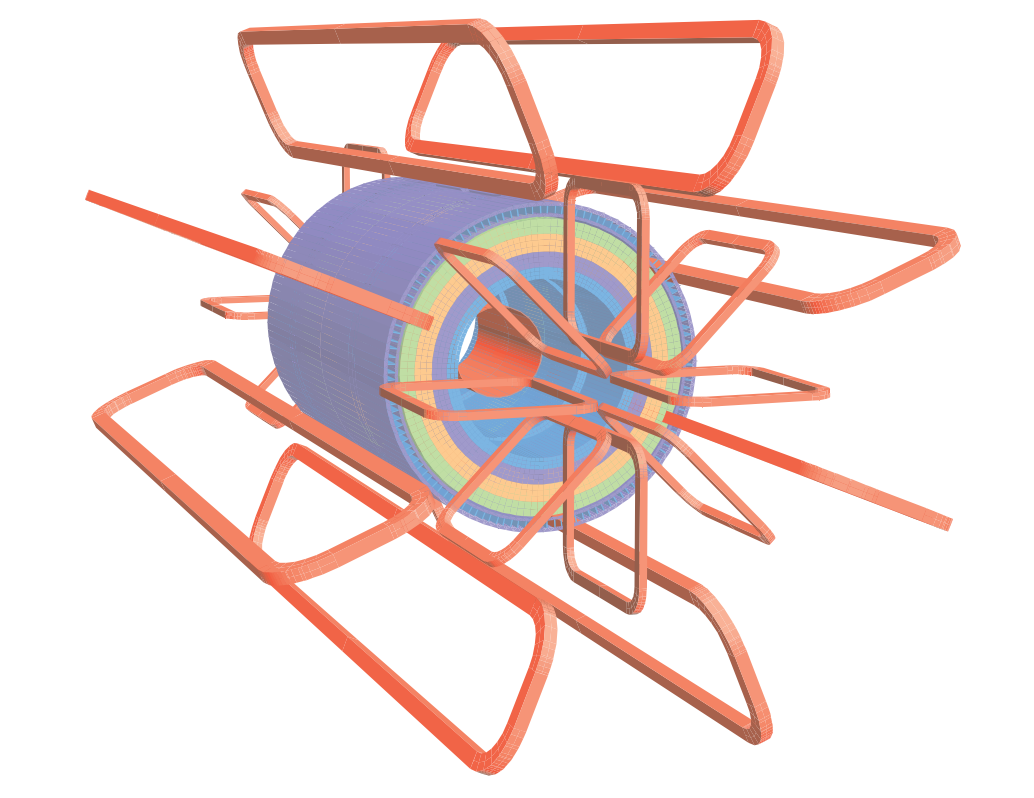
\includegraphics[width=0.475\textwidth]{Detector/MagnetSyst/magnetSyst}\label{fig:magnetSyst}}
				\hfill
				%\centering
				\subfloat[Schematic view of the superconducting magnets \cite{YAMAMOTO200853}.]
				{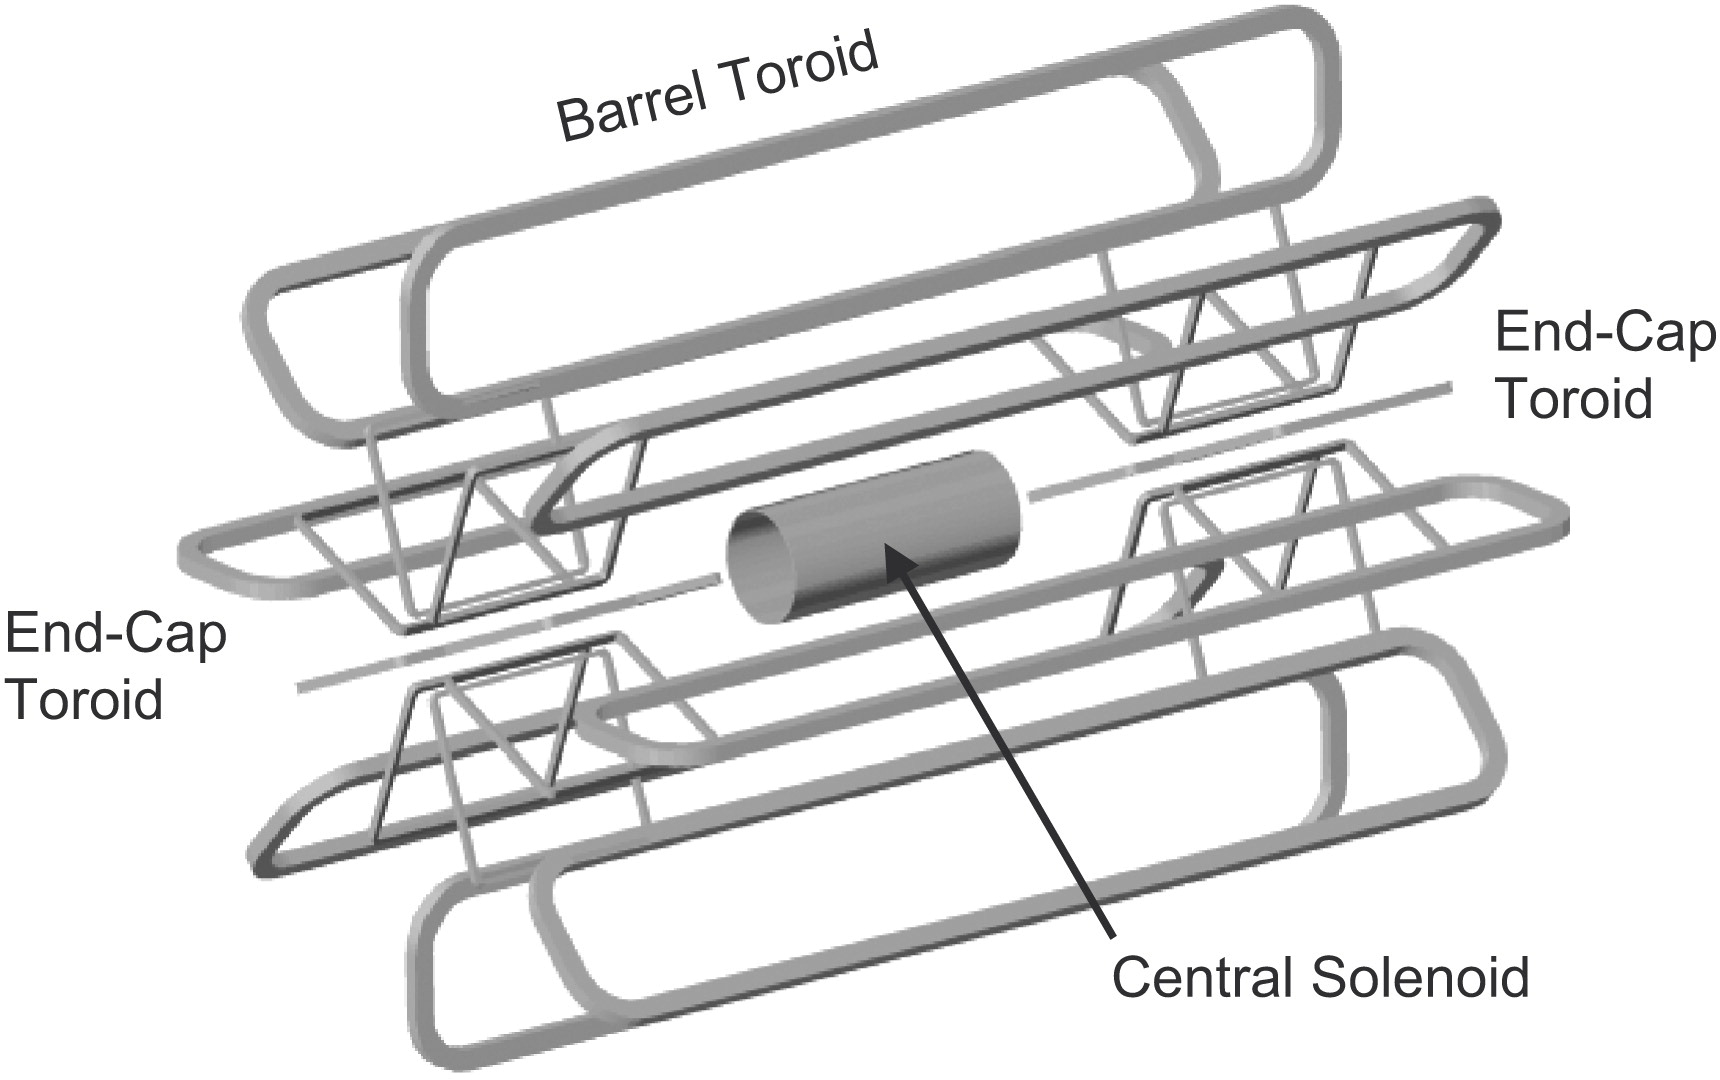
\includegraphics[width=0.475\textwidth]{Detector/MagnetSyst/magnetSyst-desc}\label{fig:magnetSyst-desc}}
				\caption{The ATLAS magnet system.}
			\end{figure}

			\noindent The ATLAS magnet system, 26 m long with a 22 m diameter, generates the magnetic field needed to bend the trajectories of charged particles in order to perform momentum measurement. Figure \ref{fig:magnetSyst} and \ref{fig:magnetSyst-desc} show the geometry of the system and its components, which are made of NbTi - superconducting material - and will be described in the following parahraphs. 



			\subsection*{The Central Solenoid}

				With an axial length of 5.8 m, an inner radius of 2.46 m, and an outer radius of 2.56 m, the central solenoid magnet is located between the ID and the ECAL. Its function is to bend the charged particles that go through the ID and it is aligned on the beam axis providing a 2 T axial magnetic field that allows accurate momentum measurement up to 100 \GeV\ \cite{YAMAMOTO200853}.

			\subsection*{The Barrel and the End-cap Toroids}

				Figure \ref{fig:magnetSyst-desc} displays the toroid magnetic system that surrounds the calorimeters. With its cylindrical shape this component consists of a barrel and two end-caps toroids, each with eight superconducting coils. The system allows accurate measurement of muon momenta using a magnetic field of approximately 0.5 T (barrel) for the central regions and 1 T (end-cap) for the end-cap regions, respectively, which bends the particles in the $\theta$ direction.

				
		% --------------------------------
		% -------  THE ID
		% --------------------------------
		\subsection{The Inner Detector}
		\label{sec:ID}

			The Inner Detector (ID) \cite{ATLASInDet} is the innermost component of the ATLAS detector \ie\ the nearest sub-detector to the interaction region and it is used to reconstruct charged particle tracks used in the selection of physics objects. In fact, it allows robust track reconstruction, with accurate impact parameter resolution ($\sim 20 \mu m$) and precise primary and secondary vertex reconstruction for charged particles (tracks) above 500 \MeV\ and within $\displaystyle|\eta| < 2.5$.

			\begin{figure}[!htb]
				\subfloat[Overview of the ATLAS ID with labels and dimensions.]{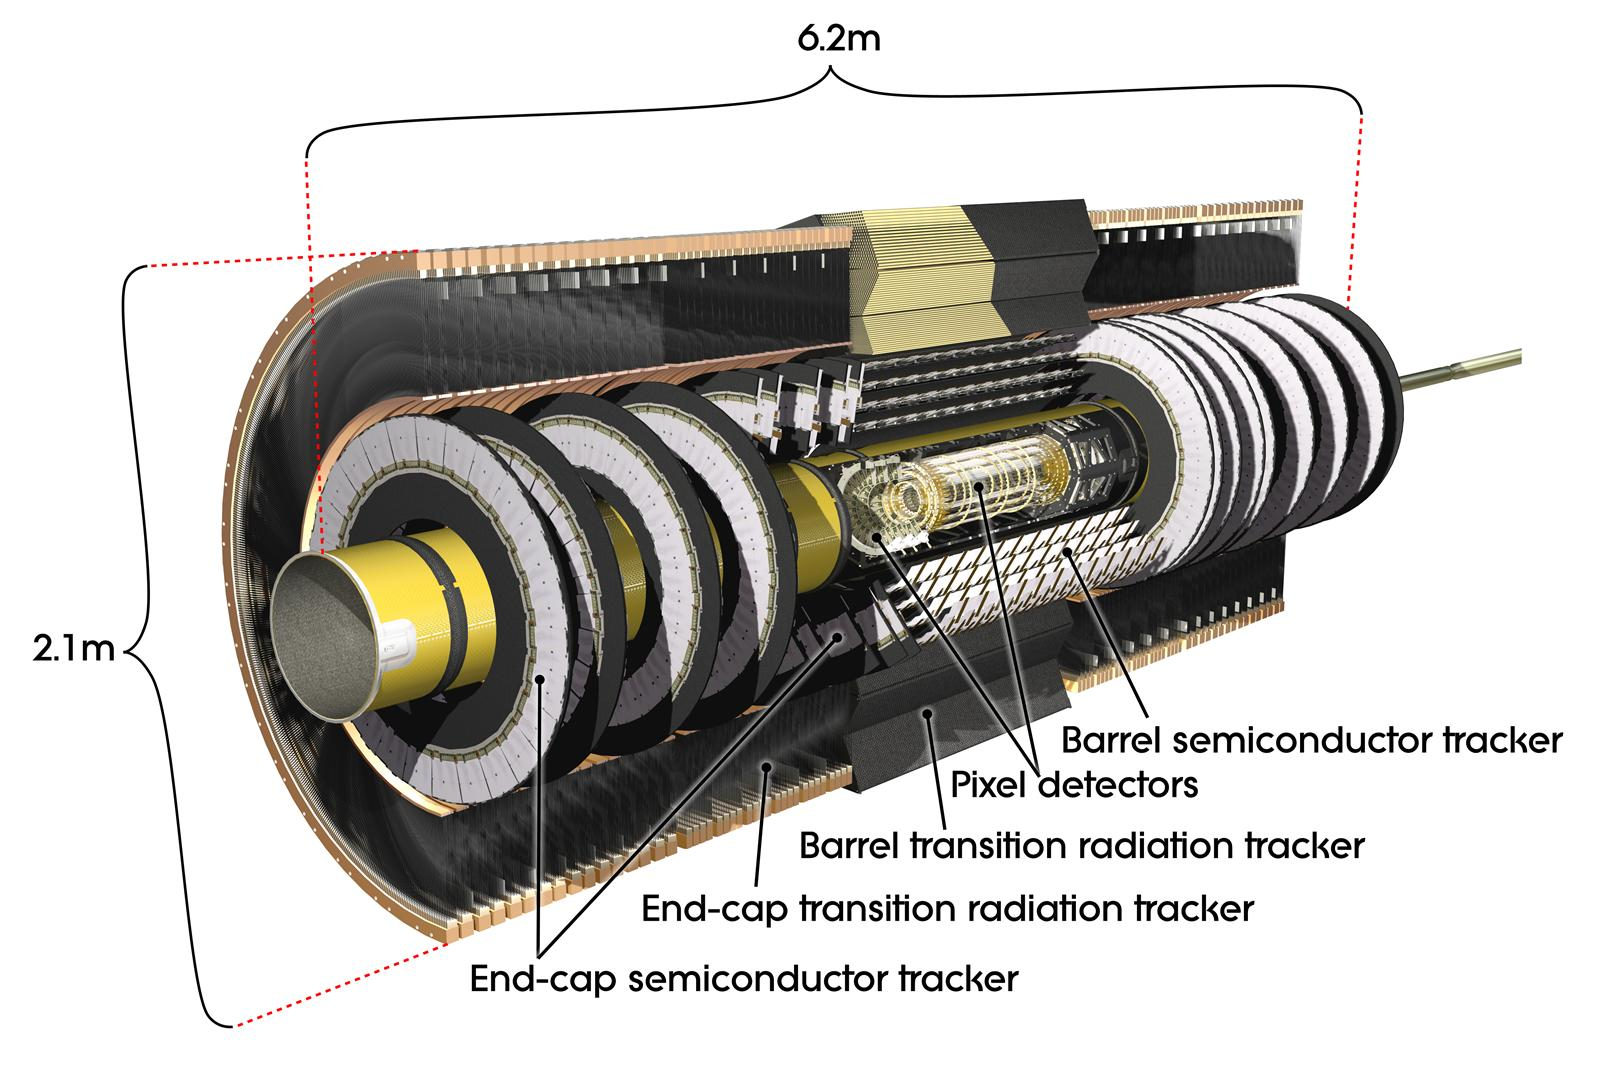
\includegraphics[width=0.475\textwidth]{Detector/ID/ID-overview}\label{fig:ID-overview}}\hfill
				\subfloat[Diagram of the ATLAS ID and its sub-detectors.]{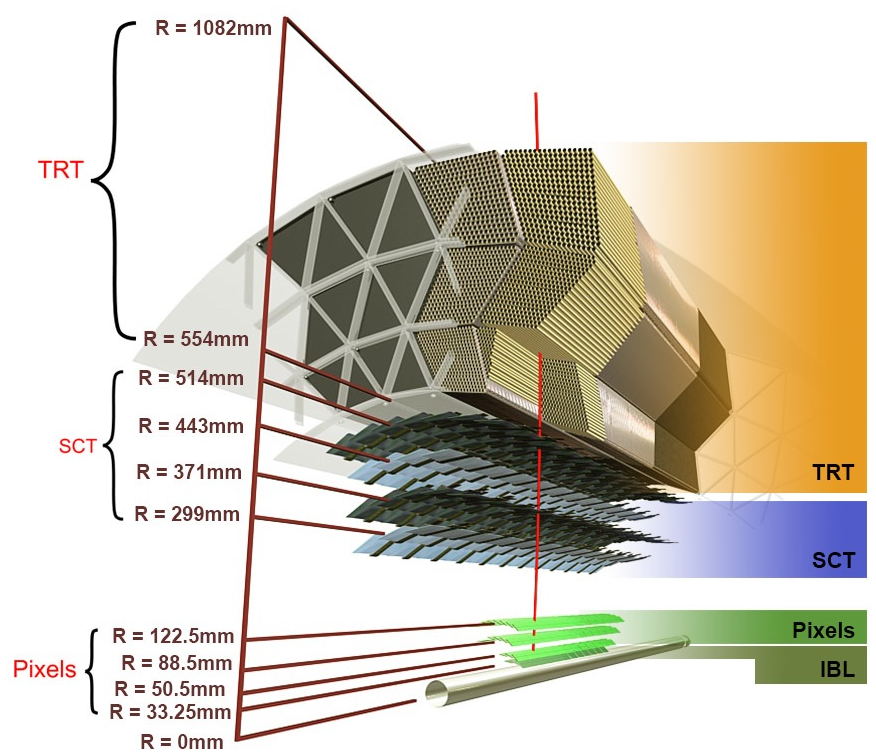
\includegraphics[width=0.475\textwidth]{Detector/ID/ID}\label{fig:ID}}
				\caption{The ATLAS Inner Detector}
				\label{fig:AID}
			\end{figure}


			The ID is comprised of independent and concentric sub-systems, which are all shown in Figure \ref{fig:AID}: %\ref{fig:ID} and \ref{fig:ID-overview}:

			\begin{itemize}
				\item \underline{Insertable B-Layer (IBL):} \\innermost Pixel Detector layer added during ATLAS Run-2 upgrade (2013/2014) to improve vertexing and impact parameter reconstruction;
				\item \underline{Silicon Pixel Tracker (Pixel):} \\made of silicon pixel layers and used mainly for reconstructing both the primary and secondary vertices in an event;
				\item \underline{SemiConductor Tracker (SCT):} \\comprised of silicon microstrip layers; thanks to its resolution ($17 \times 580\, \mu$m) it can accurately measure particle momenta;
				\item \underline{Transition Radiation Tracker (TRT):} \\final layer comprised of various layers of gaseous straw tube elements surrounded by transition radiation material.
			\end{itemize}

			These sub-detectors will be discussed in the following sections.  

			\subsection*{IBL} 
				
				The IBL \cite{IBLTDR} is the innermost Pixel Detector layer as shown in Figure \ref{fig:ID}. It is comprised of 6M channels and each pixel measures $50 \times 250\,\mu$m. Its resolution is $8 \times 40\, \mu$m,The addition of this new layer brought a considerable improvement on the performance of the Pixel Detector by enhancing the quality of impact parameter reconstruction of tracks. In particular, this was achieved by improving the vertex finding efficiency and the tagging of bottom-quark-initiated jets (\emph{b}-jets) which, in case of a B-layer failure, can be restored by the IBL. Besides these improvements, the IBL insertion allowed ATLAS to better cope with high luminosity effects such as the increase in event pile-up, which leads to high occupancy and read-out inefficiency. 

			\subsection*{Pixel}
				
				The Pixel detector is comprised of 1750 identical sensorchip-hybrid modules, each covering an active area of 16.4 $\times$ 60.8 mm. The total number of modules correspond to roughly 80 million semiconductor silicon pixels. The nominal pixel size is 50 $\mu$m in the $\phi$ direction and 400 $\mu$m in the barrel region, along the $z$-axis (beam axis) \cite{ATLASPix}. The reason why such a large amount of pixels is employed is justified by the need to cope with the high luminosity in ATLAS. The silicon pixel detector measures 48.4 cm in diameter and 6.2 m in length providing a pseudorapidity coverage of $\left|\eta\right| < 2.5$. Figure \ref{fig:ID} shows the three concentric barrel layers placed at 50.5 mm, 88.5 mm and 122.5 mm respectively. Furthermore, the Pixel detector is made of six disk layers, three for each forward region, such that when a charged particle crosses the layers it will generate a signal at least in three space points. The fine granularity of such detector allows accurate measurement and precise vertex reconstruction, as it provides a more accurate position measurement as a large detection area is available. In particular, it has a resolution of $10 \times 115\,\mu$m.

			\subsection*{SCT}

				The SCT is made of 4088 modules of silicon micro-strip detectors arranged in four concentric barrel layers. It is mainly used for precise momentum reconstruction over a range $\left|\eta\right| < 2.5$ and it was designed for precision measurement of the position using four points (corresponding to eight silicon layers), obtained as track hits when crossing the layers. Figure \ref{fig:ID} shows the structure of the SCT with its four concentric barrel layers with radii ranging from 299 mm to 514 mm and two end-cap layers. Each module has an intrinsic resolution of 17 $\mu$m in the $R-\phi$ direction and 580 $\mu$m in the $z$ direction. As the SCT is further away from the beam-pipe than the Pixel detector, it has to cope with reduced particle density. This allows for reduced granularity mantaining the same level of performance of the Pixel detector: SCT can use $\sim$ 6.3 million read-out channels.%, almost 2 million fewer than the pixel detector.


			\subsection*{TRT}
			 
				The last and outermost of the sub-systems in the ID is the TRT. It is a gaseous detector which consists of 4 mm diameter straw tubes wound from a multilayer film reinforced with carbon fibers and containing a 30 $\mu$m gold plated tungsten wire in the center. The straw is filled with a gas mixture of 70\% Xe, 27\% CO$_2$ and 3\% O$_2$ \cite{TRT2012}. As shown in Figure \ref{fig:ID}, its section consists of three concentric layers with radii ranging from 544 mm to 1082 mm, each of which has 32 modules containing approximately 50,000 straws, 1.44 m in length, aligned parallel to the beam direction with independent read-out at both ends. Both end-cap sections are divided into 14 wheels, with roughly 320,000 straws in the R-direction. The average 36 hits per track in the central region of the TRT allow continuous tracking to enhance pattern recognition and momentum resolution in the $\left| \eta \right| < 2.5$ region. It also improves the \pt\ resolution for longer tracks.



		% --------------------------------
		% -------  THE CALORIMETERS
		% --------------------------------
		\subsection{The Calorimeters}

			\begin{figure}[!htb]
				\centering
				\includegraphics[width=\textwidth]{Detector/Calo/Calo-overview}
				\caption{A computer generated image of the full calorimeter.}
				\label{fig:Calo}
			\end{figure}

			The ATLAS Calorimeter system, shown in Figure \ref{fig:Calo}, is comprised of two main sub-systems; the electromagnetic calorimeter (ECAL) and hadronic calorimeter (HCAL), which are designed to stop and measure the energy of electromagnetic-interacting and hadronic particles respectively. The combination of the two provides full coverage in $\phi$ and $\left | \eta \right | < 4.95$. Particles slow down and lose energy generating showers when crossing different layers. The ECAL is comprised of one barrel and two end-cap sectors employing liquid Argon (LAr). The showers hereby develop as electrons pairs which are then collected. The HCAL is also comprised of one barrel and two end-cap sectors. The sensors in the barrel of the HCAL are tiles of scintillating plastic whereas LAr is employed for the end-cap. A forward region, the closest possible to the beam, is covered by a LAr forward calorimeter (FCal). The LAr and Tile Calorimeter will be briefly discussed in the following parapgraphs. 
			%The particles have to deposit all their energy within the calorimeters to obtain an accurate energy measurement and avoid energy deposits in the outer muon spectrometer.
			%The definitions of radiation length ($X_0$), the distance over which an electron loses 1/$e$ of its energy within a given material, and nuclear interaction length ($\lambda_I$), are used to define the lengths of the barrel and the endcap regions of the calorimeter system. The ECAL roughly measures 22 $X_0$ thick in the region of barrel, and 24 $X_0$ in the end caps. The HCAL roughly measures 10 $\lambda_I$. Both ECAL and HCAL measures vary with $\eta$. Furthermore, it is known that hadronic particles are more penetrating than the electromagnetic ones and in particular, $\lambda_I$ is roughly ten times bigger than $X_0$. 

			\subsection*{The Liquid Argon Calorimeters}

 				The ECAL is comprised of multiple layers of liquid Argon (LAr) sampler and lead absorber. The choice of its accordion-geometry design brought two main advantages; full $\phi$ coverage with no non-interactive regions (no cracks); fast extraction of signals coming from both front or rear end of the electrodes. It is made of two half-barrel wheels, both placed in the barrel cryostat, that provide a pseudorapidity coverage up to $\left | \eta\right | < 1.475$ and two end-cap detectors providing $1.375 \leq \left|\eta\right| \leq 3.20$ coverage in two end-cap cryostats. The junction between the barrel and end cap components defines the crack region and any signal coming from the crack region is therefore discarded. 

 				In the $\left | \eta\right | < 1.8$ region there is an additional layer, placed at the front of the calorimeter, that is made of a thin (0.5 cm in the end-cap and 1.1 cm in the barrel) LAr layer with no absorber \cite{ATLASLAR}. This additional layer was designed to correct for the energy lost, as particles enter the calorimeter, by taking a measurement just before the majority of the electomagnetic shower is developed.

 				% In the barrel, the accordion layers are axial and run in $\phi$, the folding angles of the layers vary with radius to keep the liquid-argon gap constant. 
 				% In the end-caps the layers are parallel to the radial direction and run axially. 
 				% The LAr is ionised by electromagnetic showers. The read-out circuits are made of three copper layers insulated by two layers of polyimide. 
 				% The two outer layers, split in sectors, are connected to high-voltage sources and polarize the LAr gap to the absorber. 
 				% The inner layer is where the signal is collected through capacitive coupling and is then segmented into read-out pads.

			\subsection*{The Tile calorimeter}

				The main purpose of the hadronic calorimeter is to measure the energy of hadronic showers. It is built employing steel and scintillating tiles coupled to optical fibres which are read out by photo-multipliers. As shown in Figure \ref{fig:Calo}, the HCAL is made up of three cylinders; a central barrel, 5.64 m long covering a region $\left | \eta \right | < 1.0$, and two extended barrel, 2.91 m long covering a reigon $0.8 < \left | \eta \right | < 1.7$. Each cylinder is made up of 64 modules and each module is in turn made up of three layers. Ultimately, the smallest section of the calorimeter module is a cell with a $\Delta \phi \times \Delta \eta = 0.1 \times 0.1$ granularity for the two innermost layers and $\Delta \phi \times \Delta \eta = 0.2 \times 0.1$ for the outermost one. 

		% --------------------------------
		% -------  THE MU SPEC
		% --------------------------------
		\subsection{The Muon Spectrometer}
		\label{sec:MuSpec}

			The MS \cite{MSTDR}, shown in Figure \ref{fig:MS}, is the outermost sub-system of the whole ATLAS detector. As such, it surrounds the calorimeters and its main function is to perform precision measurement of muons momenta. The deflection of muon tracks employing large superconducting air-core toroid magnets and high-precision tracking chambers is at the heart of such high precision measurement. 

			\begin{figure}[!htb]
				\centering
				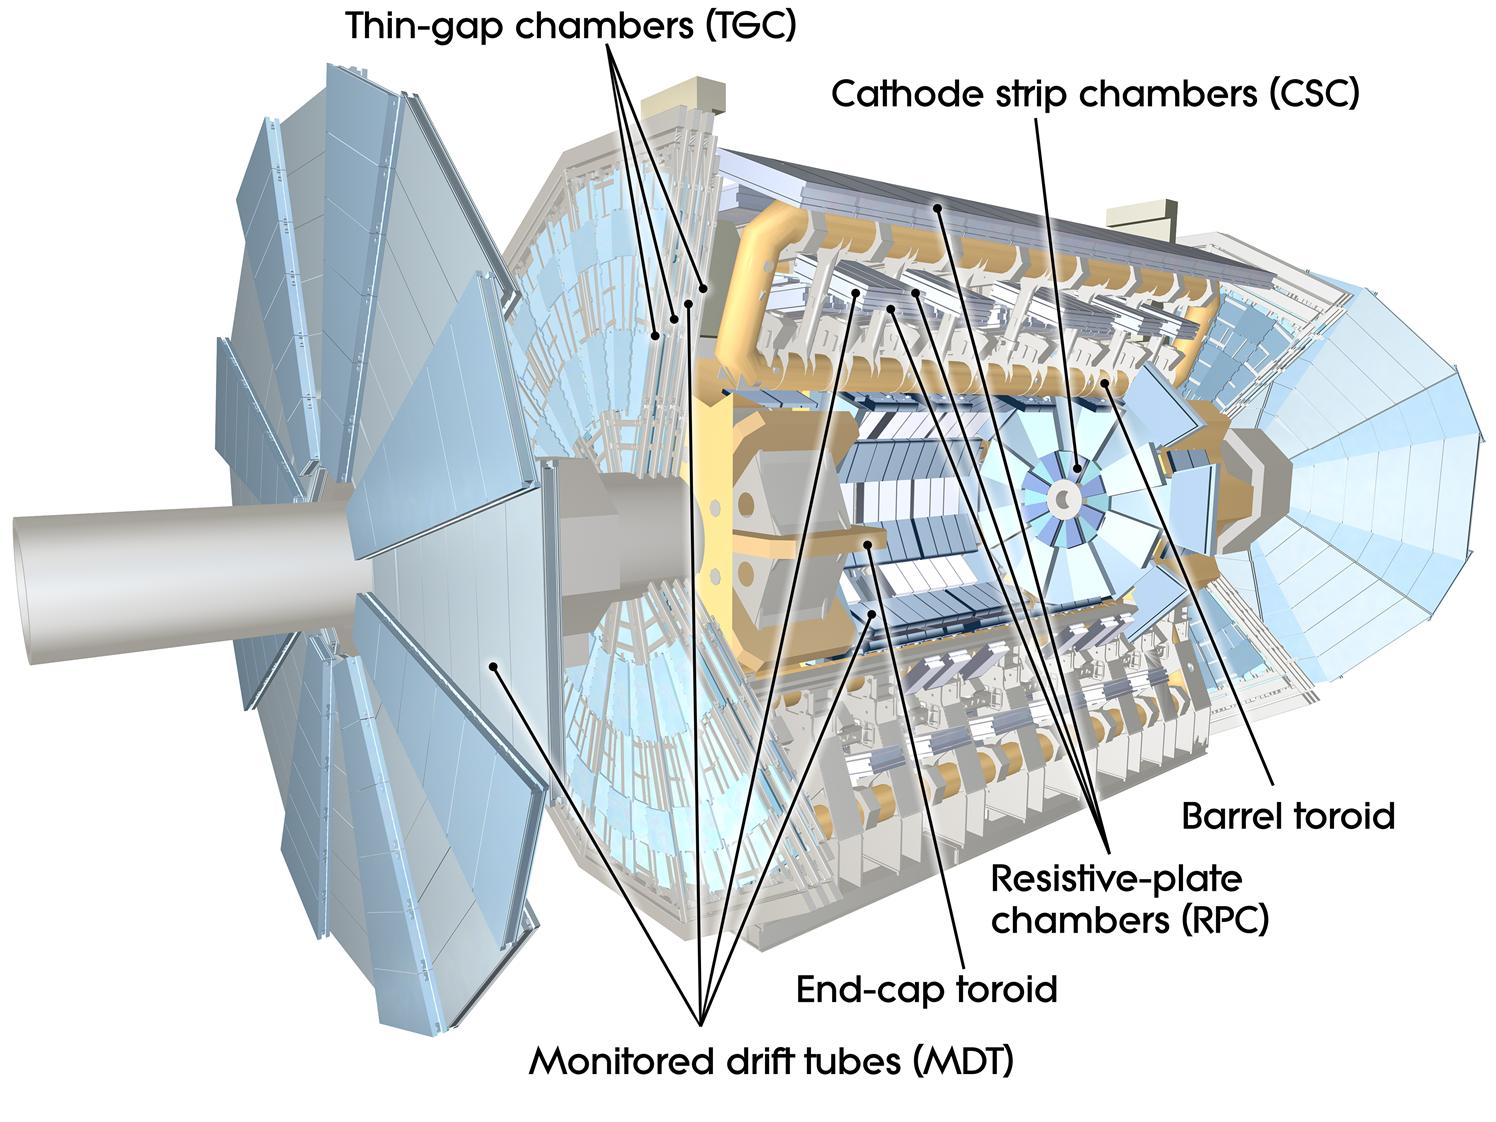
\includegraphics[width=\textwidth]{Detector/MS/MS}
				\caption{Cut-away view of the ATLAS muon system \cite{ATLASJINST}.}
				\label{fig:MS}
			\end{figure}

			The MS is comprised of one large barrel toroid, covering the region $\left| \eta \right | \leq 1.4$, and two end-cap toroids, covering $1.6 < \left| \eta \right| \leq 2.7$ which are employed together to achieve the track-bending effect wanted. The magnitude of the magnetic field in the barrel, generated by eight large superconducting coils, ranges from 0.5 to 2 T. 

			Around the beam axis, three cylindrical layers make way for the chambers, placed in planes perpendicular to the beam, used to measure tracks. 

			Monitored Drift Chambers (MDTs) are employed over most of the pseudorapidity range to provide precision measurement of track coordinates in the bending direction. 
			Cathode Strip Chambers (CSCs) are instead employed at large pseudorapidity ($2 < \left | \eta \right | < 2.7$). 
			Finally, in the end-cap regions Thin-Gap Chambers (TGCs) together with Resistive-Plate Chambers (RPCs) are dedicated to the Trigger System discussed in Section \ref{sec:trigSyst}. 


	% --------------------------------
	% -------  THE TRIGGER
	% --------------------------------
	\section{The ATLAS Trigger System}
	\label{sec:trigSyst}

		\begin{figure}[!htb]
			\centering
			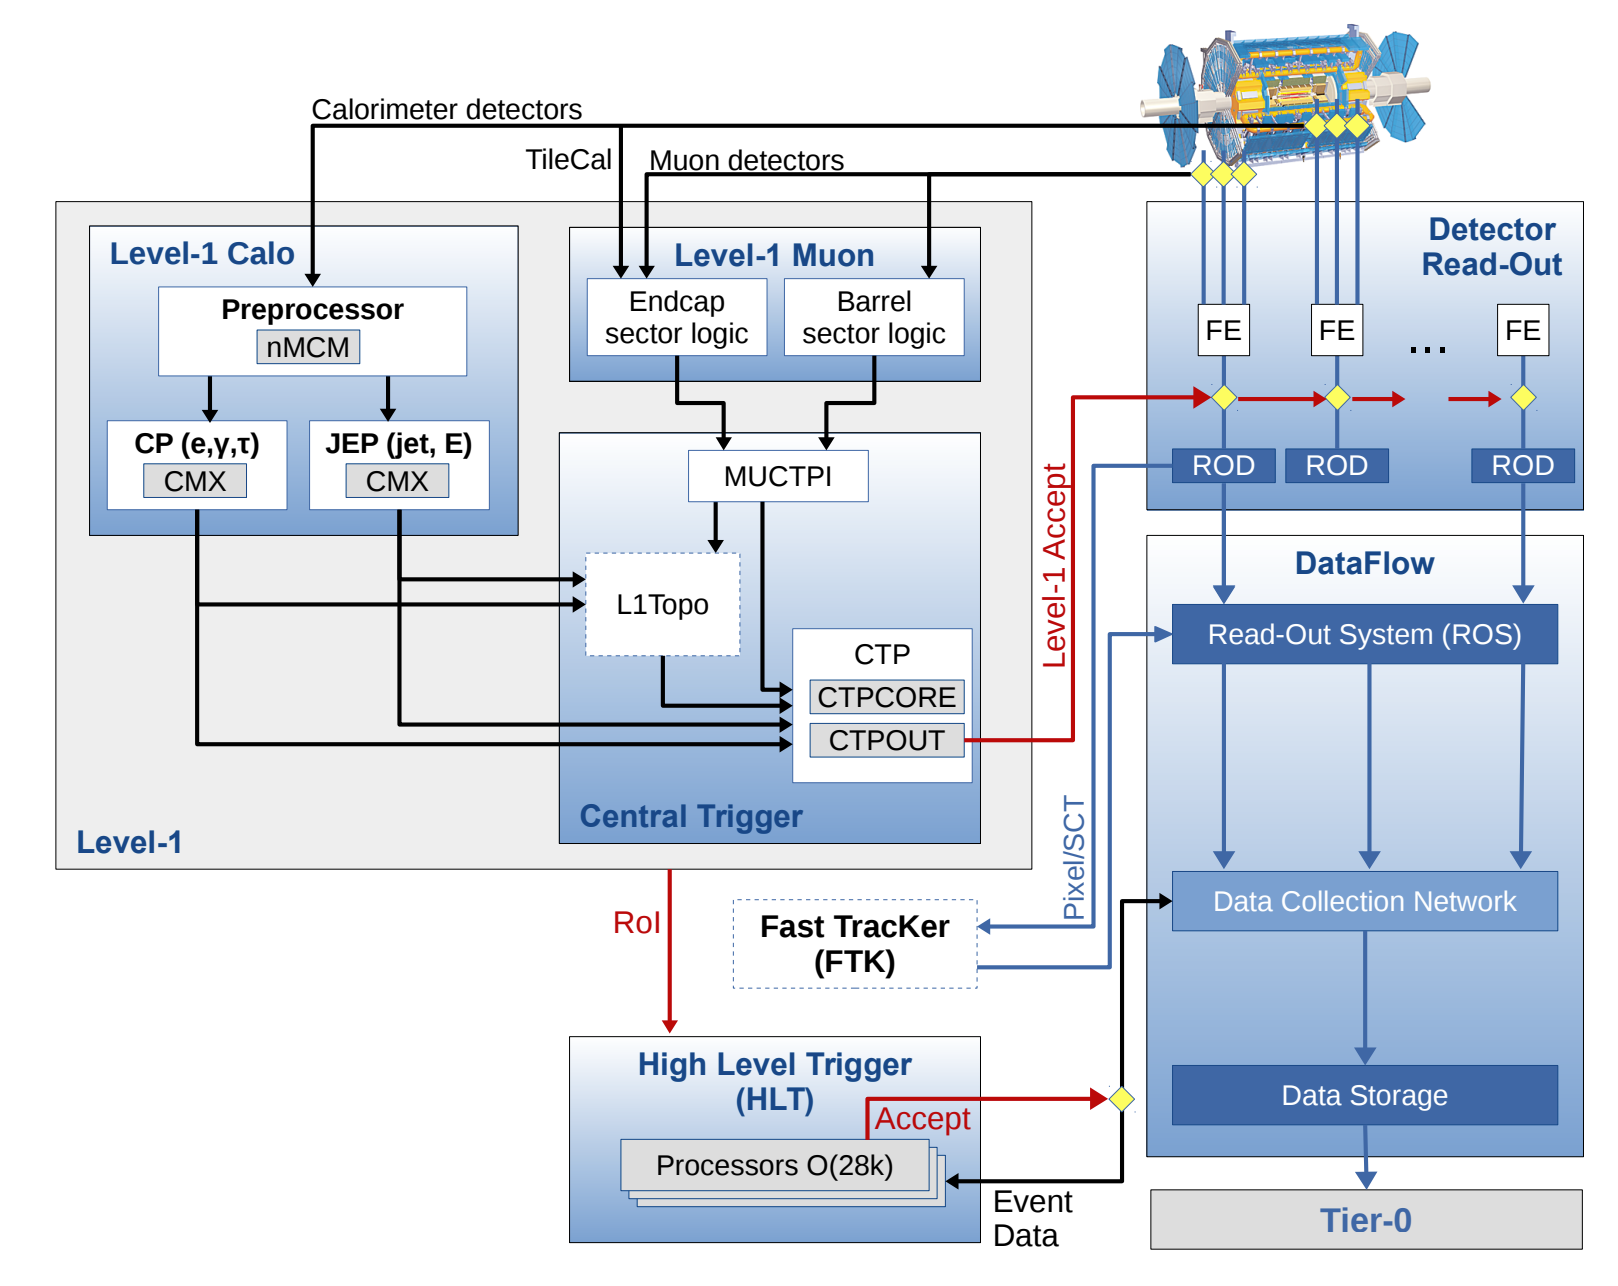
\includegraphics[width=\textwidth]{Detector/Trigger/TDAQSystem}
			\caption{The ATLAS TDAQ system. L1Topo and FTK were being commissioned during 2015 and not used for the results shown in this thesis \cite{ATLASTrigger2015}.}
			\label{fig:TDAQSyst}
		\end{figure}

		The ATLAS Trigger System is at the heart of data taking. It is an essential component of any nuclear or particle physics experiment since it is responsible for deciding whether or not to store an event for later study \cite{ATLASTrigger2015}. The ATLAS Trigger system is employed to reduce the event rate from $\sim$ 40 MHz\footnote{The LHC delivers beams with a bunch-spacing of 25 ns.} bunch-crossing\footnote{The term bunch-crossing is hereby used when referring to a collision between two bunches of protons. Since only a certain fraction of the total momentum carried by each proton contributes to the collision, an average number of interactions per bunch-crossing, $\left < \mu \right >$ is used.} to $\sim$ 200 Hz which corresponds to roughly 300 MB/s.

		The Trigger and Data Acquisition (TDAQ) system shown in Figure \ref{fig:TDAQSyst} consists of a hardware-based first level trigger (L1) and a software-based high-level trigger (HLT). The L1 trigger decision is formed by the Central Trigger Processor (CTP), which receives inputs from the L1 calorimeter (L1Calo) and L1 muon (L1Muon) triggers. The first level (L1), which was designed to perform the first selection step, is a hardware-based system that uses information from the calorimeter and muon subdetectors. It also defines the so-called Regions of Interest (RoIs) within the detector to be investigated by the next level trigger, the HLT. Additionally, a Fast TracKer (FTK) system \cite{FTKTDR} (not yet installed) will provide global ID track reconstruction at the L1 trigger rate using lookup tables stored in custom associative memory chips for the pattern recognition. The FPGA-based track fitter will perform a fast linear fit and the tracks are made available to the HLT. This system will allow the use of tracks at much higher event rates in the HLT than is currently affordable using CPU systems. However, the upgrade of the ATLAS trigger will not be discussed any further.

		In the next sections the L1 and HLT will be briefly described. 


		\subsection{Level 1 Trigger}

			The Level 1 Trigger identifies Regions of Interest (RoIs)\footnote{$\eta - \phi$ regions where event features have been fouind by the L1 selection process.} and passes these to HLT which will perform further investigations. Furthermore, in order to decide whether or not the event processing will continue, L1 selection uses only information coming from some parts of the detector to keep the input rate to a maximum of 100 kHz. L1 is implemented in fast custom electronics to keep the latency\footnote{Time needed by an electric signal to get to the front-end electronics.} below $2.5\, \mu$s. Event data from other sub-sytstem are temporarily stored in memories whilst L1 decision is taken. 

			The L1 topological trigger (L1-Topo) \cite{ATLASL1Topo} is feeded with energy and direction information, about the objects found by the L1 calorimeter and the muon trigger, which will be processed by dedicated algorithms implemented in its own FPGAs. However, due to the 100 kHz read-out rate, not all the information collected by L1-Topo will be sent to the HLT, but only part of it. In order to properly seed the RoI-guided HLT reconstruction, speficic objects in combination with the correct topological criteria must be employed.


		\subsection{High-Level Trigger}

			The HLT is used to reduce the output rate down to 1 kHz and it has a $\sim$200 ms average decision time. Events that pass L1 trigger are then processed by the HLT using finer-granularity calorimeter information, precision measurements from the MS and tracking information from the ID. The HLT reconstruction can be run within RoIs identified at L1 or a so-called full-scan on the full detector can be performed. The track reconstruction in the Inner Detector is an essential component of the trigger decision in the HLT and it will be discussed more in detail in Chapter \ref{ch:trigger}







